\chapter{Results}
\label{ch:results}
The Kalman filter and controls algorithms discussed in this thesis were implemented in software on a PackBot and run in an open field with an uneven surface consisting of dirt and gravel. This testing area is difficult for the robots to navigate because pitch, roll and elevation change and the loose dirt and gravel cause the tracks to slip leading to erroneous encoder data.

*** I want to show plots with the position estimate using GPS only, KF with learned Q/R but no adapting, KF with no adapting or training, KF with adapting, KF with learned and adaptive, KF with different encoder equations. Would be cool to plot these on an overhead image of the test area. ***

*** I want to show plots of the variance of the KF position estimate and the derivative of the control outputs of linear and angular velocity. The real goal is to have smooth velocities which will show up as constant accelerations and I want to see if there is any correlation between the variance of the position estimate and the accelerations, especially when the variance of the position esimate has a large amplitude. This would indicate that the controller is not necessarily doing a poor job and I could relate this to the example of the robot controller causing the robot to spin in circles when the IMU is giving faulty outputs. Note that this would not be a sufficient condition to show that the controller is performing properly but would only be an indication that the KF output needs improvement. There are likely ways of assessing controller performance if the KF output variance is large though. ***

*** Another good set of results would be to plot the variance values returned by the GPS receiver and saved in the ACS KF log files vs the estimated variance of the KF output vs the actual error between the KF output and ground truth. ***

\section{Kalman Filter Results}
\label{sec:kfResults}
Using logged data from the Kalman filter running with default $Q$ and $R$ parameters the robot track is shown in Figure \ref{fig:kfPlainDataFirstAttempt}.

\begin{figure}[ht!]
	\centering
	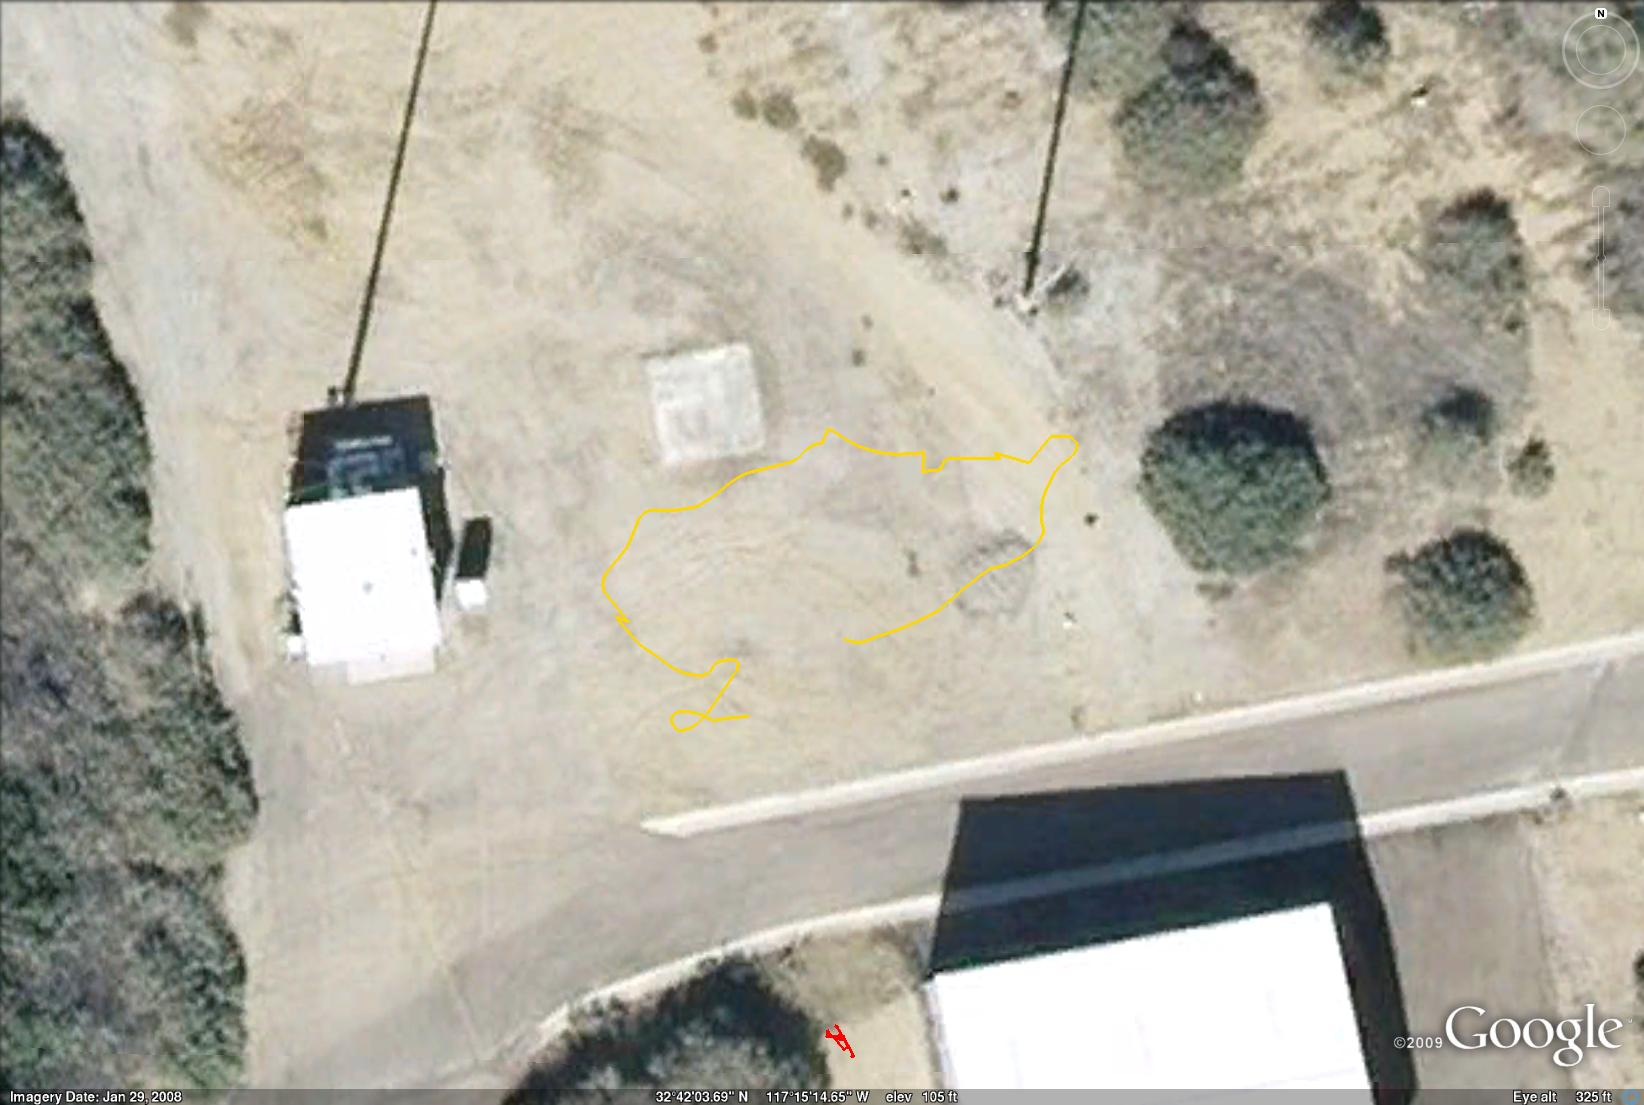
\includegraphics[width=.95\textwidth]{images/kfPlainDataFirstAttempt}
	\caption{Kalman filter output using the default parameters. The robot track is shown in yellow and a static GPS receiver with DGPS corrections is shown in red.}
	\label{fig:kfPlainDataFirstAttempt}
\end{figure}

\section{Model Based Controller Results}
\label{sec:lyapunovResults}
The control law derived in (\ref{eq:lyapunovControlLaw}) was tested in the previously described area in two different ways. The first set of results used a single set of gains and had the goal heading set to use the current heading of the robot so that $\theta^\star=\alpha$ as discussed in section \ref{sec:lyapunovVariables}. Figure \ref{fig:resultsLyapunovGEKF} shows the actual position of the robot during navigation as well as the waypoints that defined the desired route.

\begin{figure}[ht!]
	\centering
	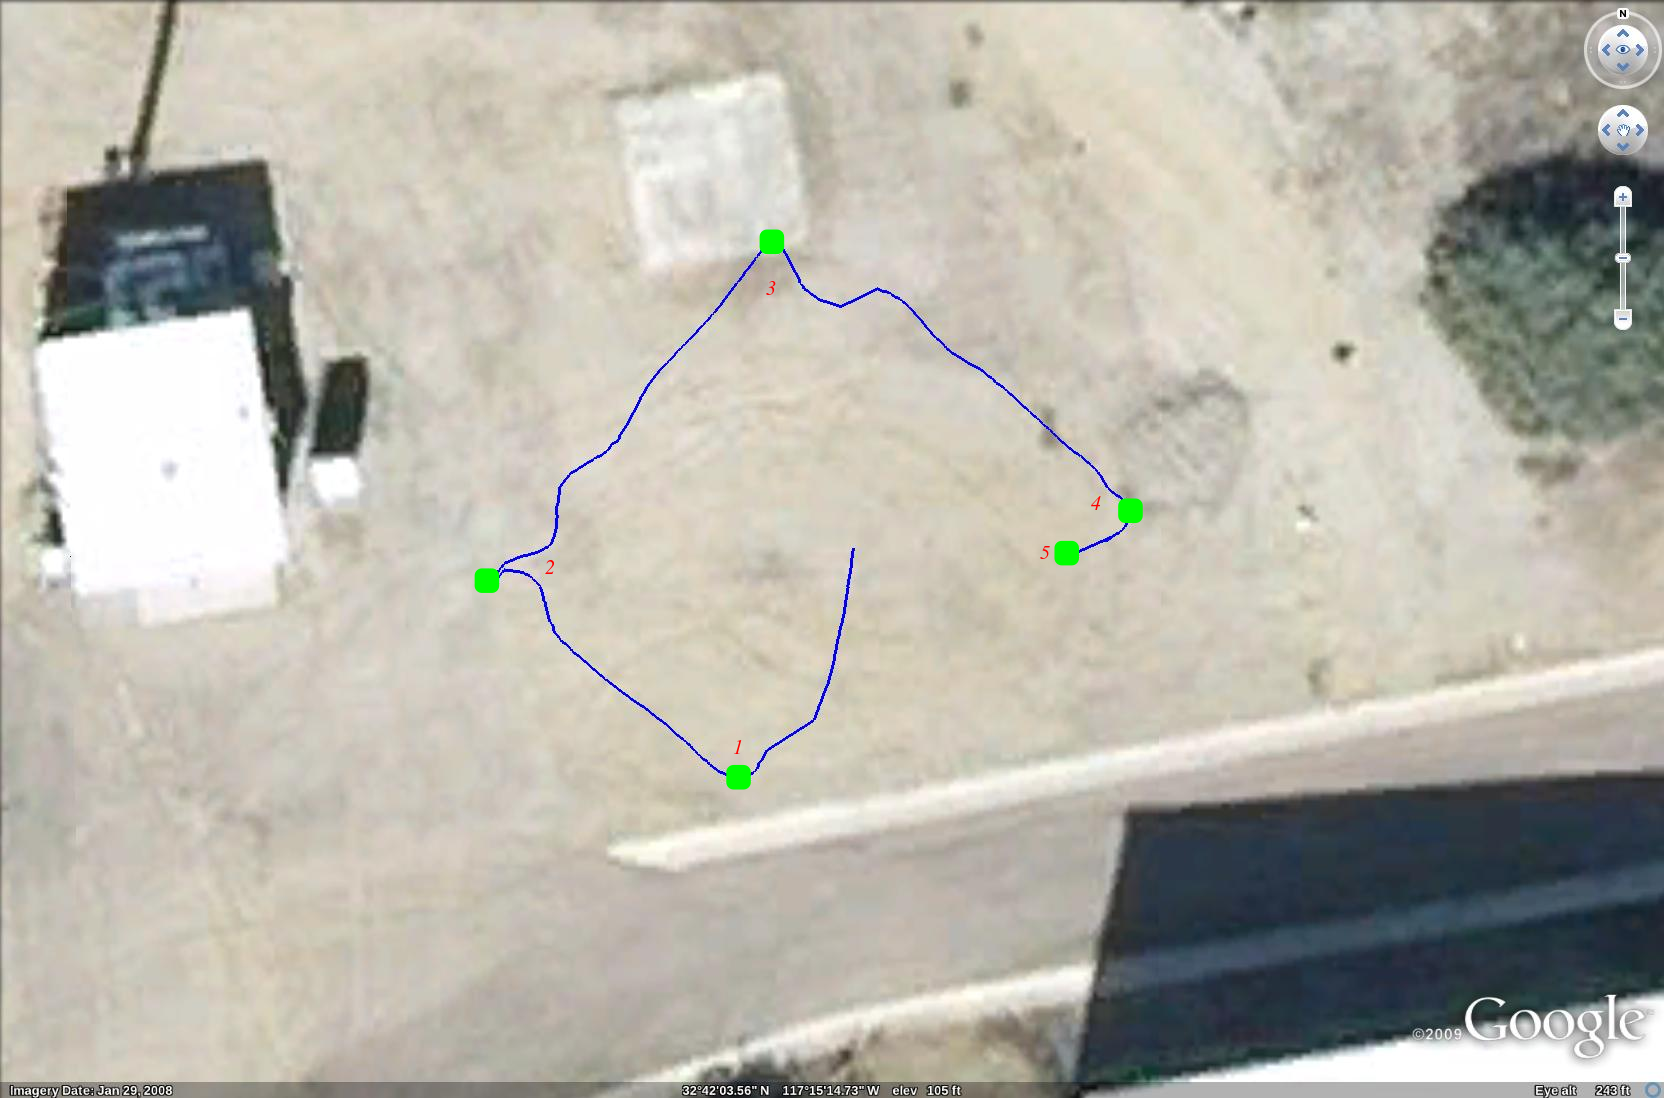
\includegraphics[width=.5\textwidth]{images/20100918_1717_GE_KF_waypts}
	\caption{Robot position during controller testing.}
	\label{fig:resultsLyapunovGEKF}
\end{figure}

Figure \ref{fig:resultsLyapunovVelocities} shows how the linear and angular velocities changed over time as measured by the Kalman filter output. The gains used were $h=0.1$, $k=0.25$ and $\gamma=0.23$. A clear deceleration can be seen as the robot approaches each waypoint although the linear velocity does not go to zero until the final waypoint due to the use of the carrot in the path planner as discussed in section \ref{sec:lyapunovVariables} for determing the error distance $e$. One of the consequences of using a model based controller is that a negative linear velocity was used after reaching the second waypoint and having the error angle $\alpha$ move towards the third waypoint which is rarely, if ever, encountered when using the original PID controller.

\begin{figure}[ht!]
	\centering
	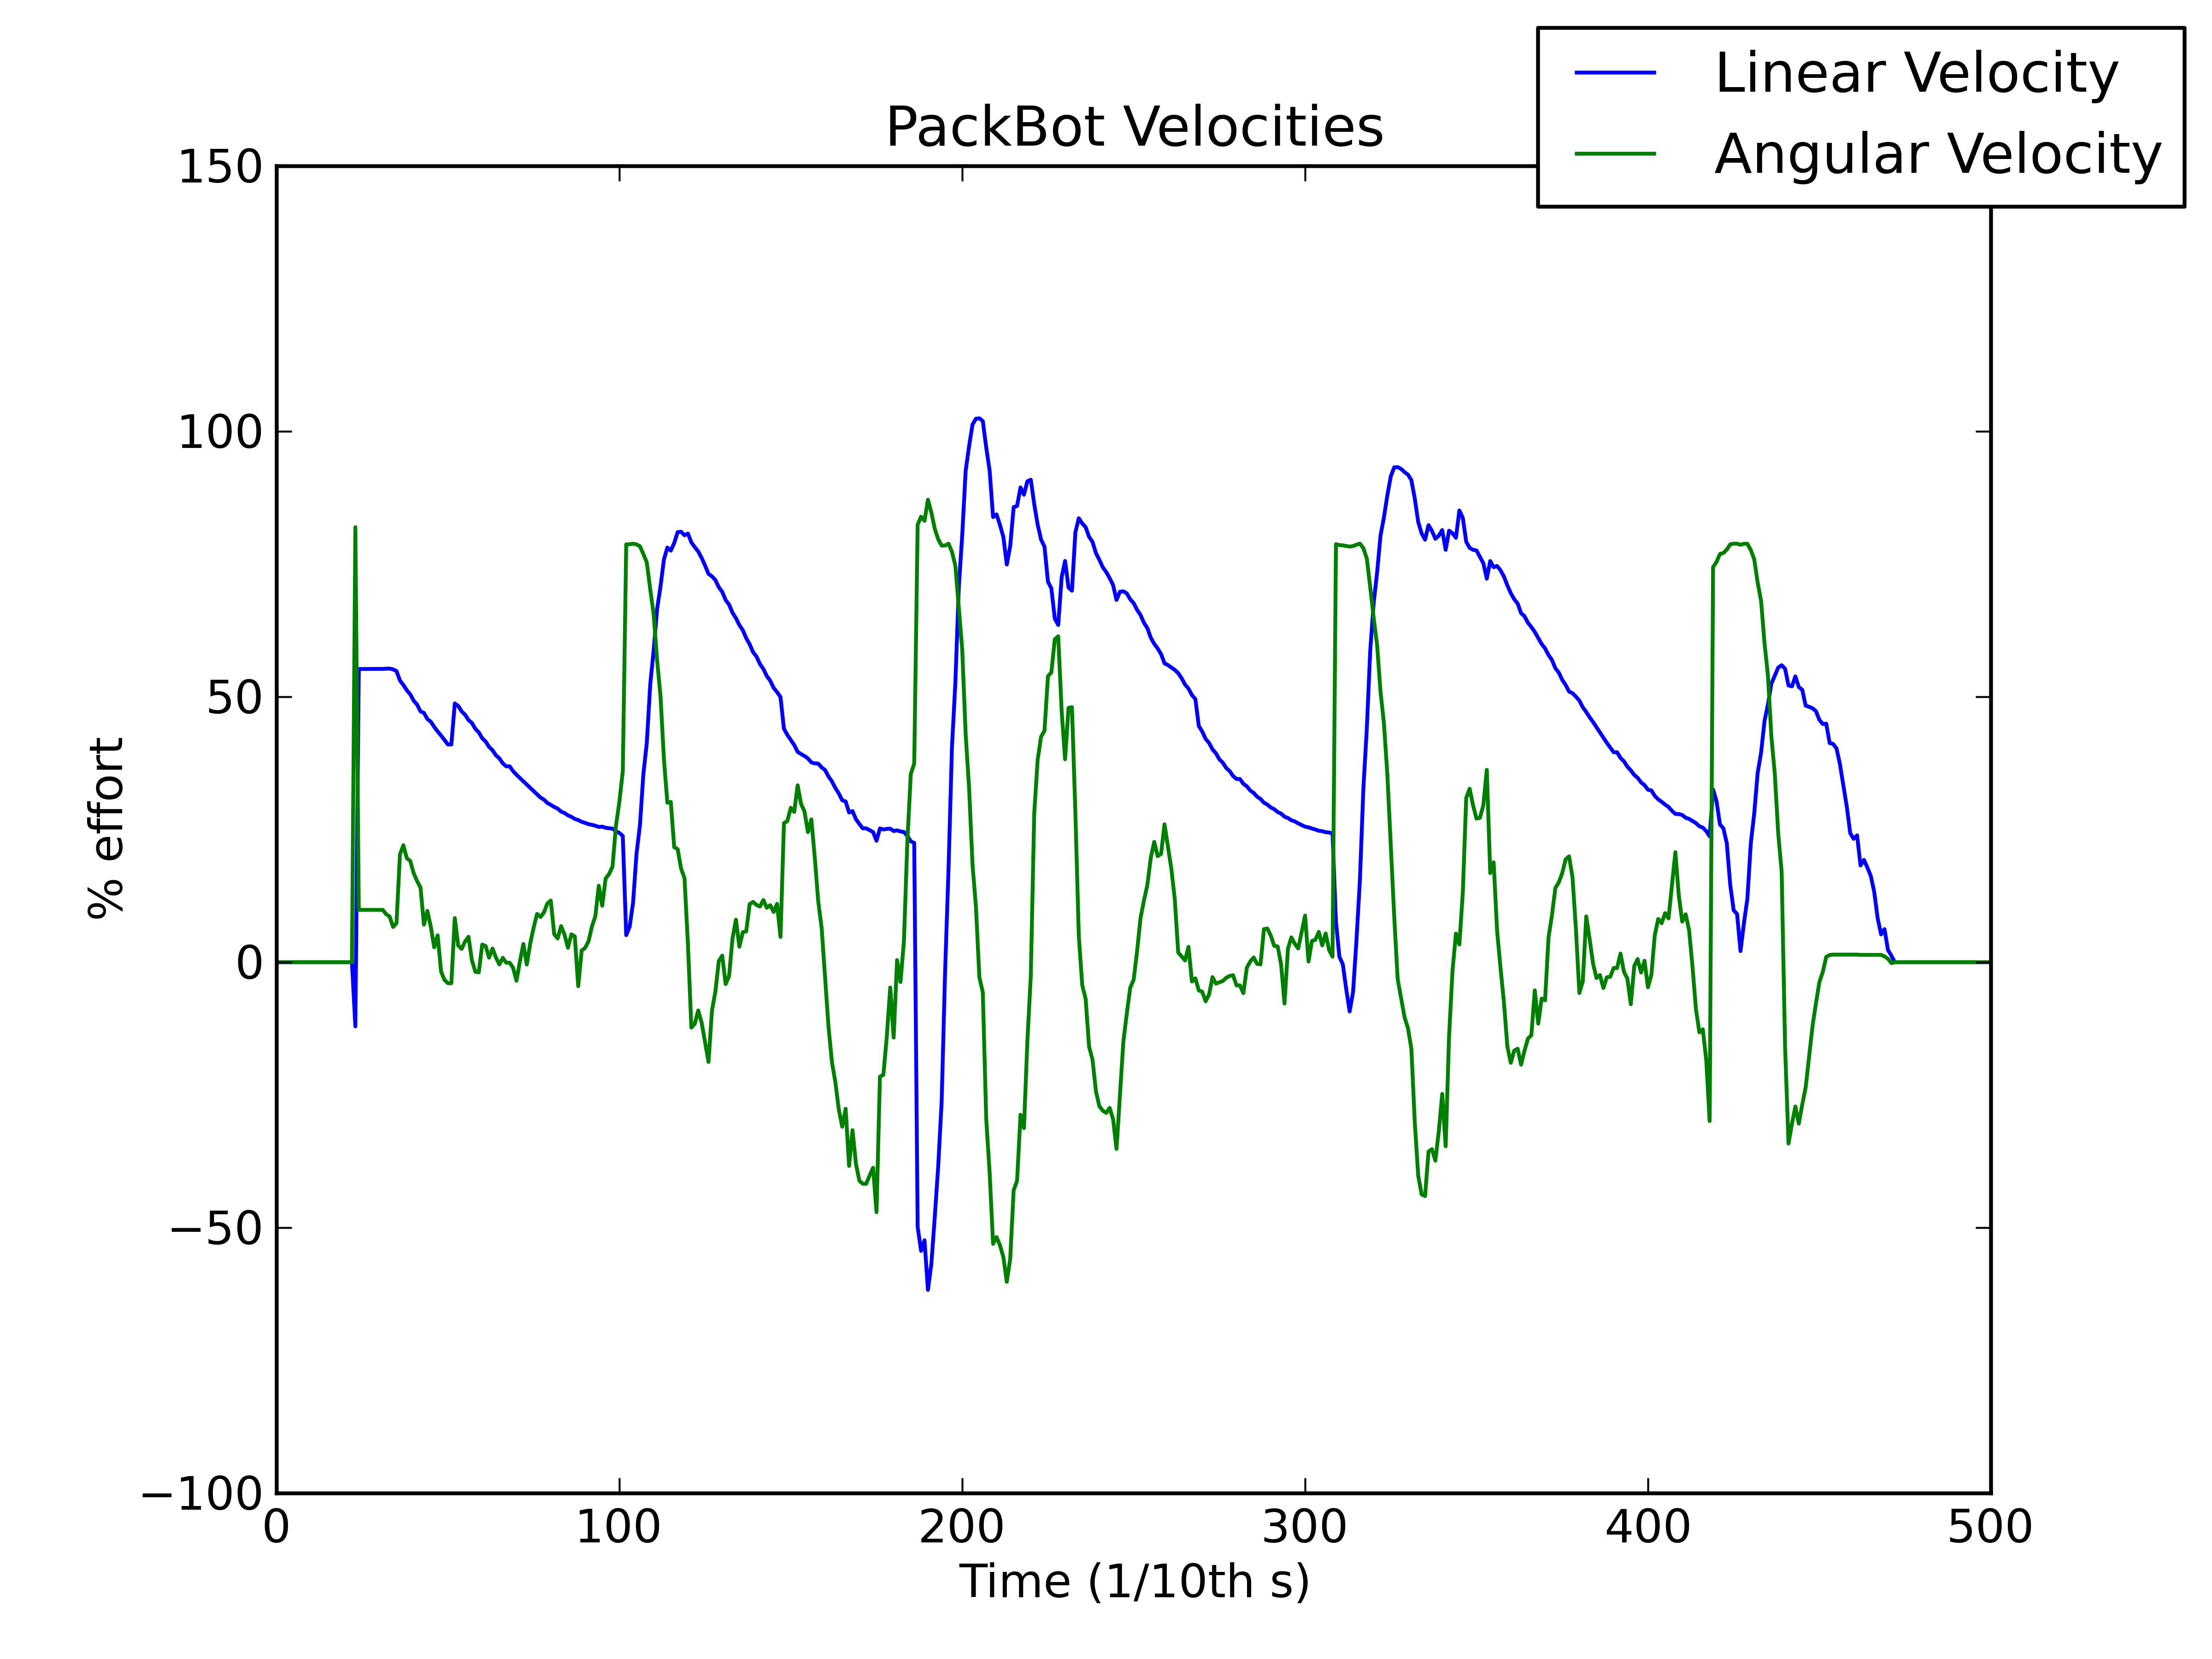
\includegraphics[width=.5\textwidth]{images/20100918_1717_velocities}
	\caption{Linear and angular velocity outputs using model based controller.}
	\label{fig:resultsLyapunovVelocities}
\end{figure}

The process of selecting gains in section \ref{sec:lyapunovTrajectoryConvergence} only applies as $(\alpha, \theta)\to(0,0)$ but says nothing about what happens when the angle errors are not small. Empirically it was determined that the gains $h=0.25$, $k=0.2$ and $\gamma=0.2$ worked well in creating smooth trajectories and later it was found that these gains cause $\zeta=1$ so that, when the angle errors are small, the system $A$ is critically damped although $\sigma>\gamma$ so the distance error converges faster than the angle errors. The best results occurred when the gains were set to $h=0.25$, $k=0.2$ and $\gamma=0.2$ \textit{until} the angle errors were $|\alpha|<0.5$ \textit{and} $|\theta|<0.5$ radians which leads to the linear approximation being valid and the gains were then changed to $h=1.1$, $k=0.42$ and $\gamma=0.2$. This second set of gains, used when the angle errors were small, are critically damped for the system $A$ since $\zeta=1$ and the angle errors converge faster than the distance error since $\sigma>\gamma$. The results of this adaptive gain scheme can be seen in Figures \ref{fig:resultsLyapunovPositionAdaptive} and \ref{fig:resultsLyapunovVelocitiesAdaptive}. Note that the goal heading, $\theta^\star$, was set to be the angle from the current waypoint to the next waypoint so that the robot would be pointing in the direction of the next waypoint when it reached the current waypoint. For the last waypoint in the route the goal heading used was $\theta^\star=\alpha$.

\begin{figure}[ht!]
	\centering
	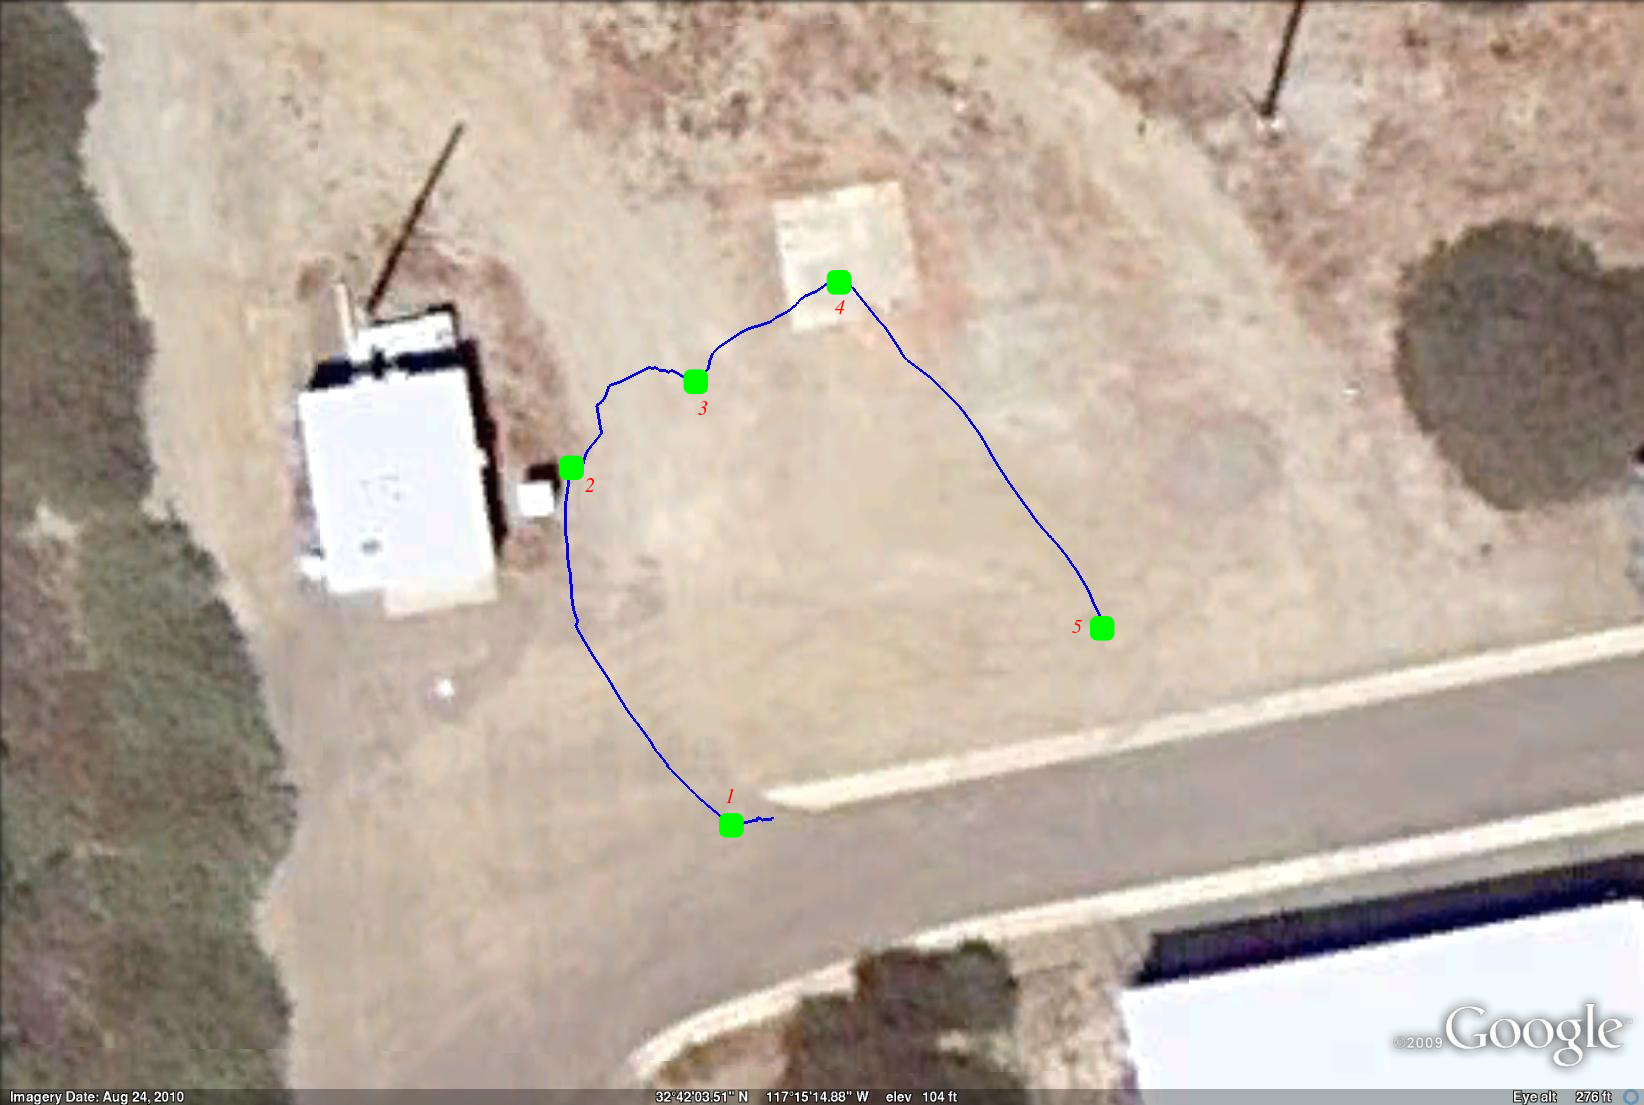
\includegraphics[width=.5\textwidth]{images/20100929_1448_GE_KF_waypts}
	\caption{Robot position using adaptive gain scheme.}
	\label{fig:resultsLyapunovPositionAdaptive}
\end{figure}

\begin{figure}[ht!]
	\centering
	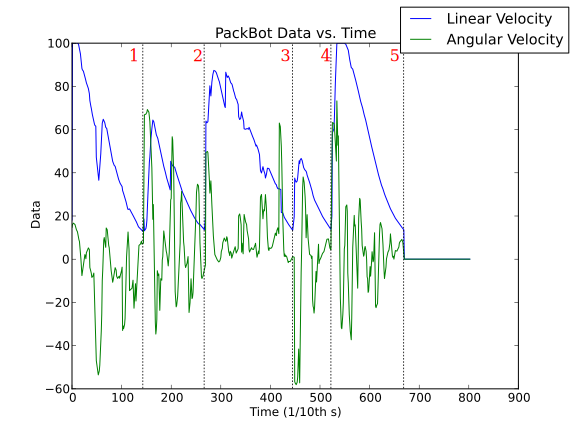
\includegraphics[width=.5\textwidth]{images/20100929_1448_pbtx}
	\caption{Linear and angular velocities with adaptive gain scheme.}
	\label{fig:resultsLyapunovVelocitiesAdaptive}
\end{figure}

\subsection{Controller Comparison}
\label{sec:controllerComparison}
For both PID (section \ref{sec:pid}, Table \ref{tab:PIDGainEffects}) and the model based controller (section \ref{sec:lyapunovTrajectoryConvergence}) gains have to be selected, the difference being that stability is the goal when selecting PID gains whereas stability is guaranteed with the model based controller. More advanced behaviors such as three point turns are a consequence of the control law in (\ref{eq:lyapunovControlLaw}) derived using a kinematic model of the robot. The other very large difference between the controllers is that a table of gains must be tuned for the PID controller to work at varying linear velocities but the model based controller works very well at different linear and angular velocities. Also, when properties of the robot such as mass are changed by using different payloads for the system the entire table of PID gains must be retuned while, at most, one set of gains must be retuned for the model based controller. This last benefit of the model based controller makes it very appealing to use in fielded systems since it reduces the amount of maintenance and effort required to keep the robot in working condition. The model based controller will also allow for improved navigation performance near obstacles which leads directly to improved autonomy for the robot.
